\chapter{Triton Kernel Profiling and Auto-tuning}\label{ch:triton}

\emph{Placement in the stack.} This chapter closes the loop. Every
earlier chapter produced a number: a throughput, a memory footprint, a
block-skip ratio, a decode speedup. Unless those numbers can be
reproduced by an independent implementation, they are not yet
engineering evidence. The pipeline described here takes every
kernel that was introduced in Chapters~\ref{ch:cutlass}--\ref{ch:sglang}
and re-implements it in Triton, measures it on the same hardware, and
reports whether the two implementations agree to within the
specified tolerance. The feedback arrow from this chapter to
Chapter~\ref{ch:distributed} in Fig.~\ref{fig:intro_stack} is
deliberate: the shape-indexed auto-tune cache developed in this
chapter is what lets the distributed-training recommendations of
Chapter~\ref{ch:distributed} remain valid as the input shape and the
hardware generation change.

This chapter describes the final layer of the software stack: a
Triton-based profiling and auto-tuning pipeline that ties together
the CUTLASS GEMM work of Chapter~\ref{ch:cutlass}, the attention
kernels of Chapters~\ref{ch:swfa} and~\ref{ch:sglang}, and the
distributed-training measurements of Chapter~\ref{ch:distributed}.
The pipeline serves two complementary purposes: it provides a uniform
measurement surface across Triton, CUTLASS, and Torch-inductor
implementations of the same kernel, and it contains an auto-tuner that
selects block sizes, warp counts, and pipeline depths as a function of
the input shape and data type.

\section{Triton Programming Model}\label{sec:triton_model}
Triton~\cite{tillet2019triton} is a Python-embedded DSL for writing
GPU kernels. A Triton program operates at the \emph{tile} level---%
unlike CUDA, where the programmer reasons about individual threads,
Triton exposes \texttt{tl.load}/\texttt{tl.store} on blocks and leaves
register allocation, shared-memory partitioning, and vectorisation to
the compiler. This makes Triton an attractive complement to CUTLASS
for rapid experimentation with GEMM, attention, and element-wise
fusion.

A minimal Triton GEMM kernel illustrates the model:
\begin{lstlisting}[language=Python,basicstyle=\ttfamily\scriptsize]
@triton.jit
def matmul_kernel(A_ptr, B_ptr, C_ptr, M, N, K,
                  BLOCK_M: tl.constexpr,
                  BLOCK_N: tl.constexpr,
                  BLOCK_K: tl.constexpr):
    pid_m = tl.program_id(0)
    pid_n = tl.program_id(1)
    offs_m = pid_m*BLOCK_M + tl.arange(0, BLOCK_M)
    offs_n = pid_n*BLOCK_N + tl.arange(0, BLOCK_N)
    offs_k = tl.arange(0, BLOCK_K)
    acc = tl.zeros((BLOCK_M, BLOCK_N), dtype=tl.float32)
    for k in range(0, K, BLOCK_K):
        a = tl.load(A_ptr + offs_m[:, None]*K + (k + offs_k)[None, :])
        b = tl.load(B_ptr + (k + offs_k)[:, None]*N + offs_n[None, :])
        acc += tl.dot(a, b)
    tl.store(C_ptr + offs_m[:, None]*N + offs_n[None, :], acc)
\end{lstlisting}
The \texttt{tl.constexpr} annotation marks parameters that are
propagated through the Triton compiler as compile-time constants, so
each $(B_m, B_n, B_k)$ triple becomes a separate kernel binary.

\section{Methodology}\label{sec:triton_method}

\subsection{Profiling Pipeline}\label{sec:triton_pipeline}
The profiling pipeline built for this thesis consists of four layers,
each addressing a distinct question about a candidate kernel.
\begin{enumerate}
    \item \textbf{Timing harness.} Each kernel is wrapped in a
          warmup/steady loop with CUDA events so that launch
          overhead is removed. Every configuration is repeated enough
          times for the standard deviation of the measured latency to
          fall below $1\%$.
    \item \textbf{Roofline analysis.} Arithmetic intensity is
          computed from the kernel's FLOP count and HBM traffic; the
          result is compared to the A100's roofline
          (FP16: $312$\,TFLOP/s, HBM: $1555$\,GB/s) to decide whether
          the kernel is compute- or memory-bound.
    \item \textbf{Nsight Compute cross-check.} For kernels that
          deviate significantly from the roofline, \texttt{ncu}
          provides occupancy, cache-hit, and stall breakdowns so that
          the root cause can be attributed to a specific hardware
          unit.
    \item \textbf{Auto-tuning.} Triton's built-in \texttt{autotune}
          iterates over block-size / num-warps / num-stages
          combinations; the best configuration is cached on disk keyed
          by input shape and data type.
\end{enumerate}

\subsection{Kernels Under Study}\label{sec:triton_kernels}
The pipeline is exercised on four representative kernels:
\begin{itemize}
    \item a dense GEMM of shape $4096 \times 4096 \times 4096$ (MLP
          projection);
    \item a Flash Attention forward pass at sequence length $2048$;
    \item the Sliding Window Flash Attention forward at sequence
          length $2048$ and window $512$
          (Chapter~\ref{ch:swfa});
    \item the SGLang decode-attention kernel at KV length $8192$
          (Chapter~\ref{ch:sglang}).
\end{itemize}
Each is implemented three times (Triton, CUTLASS, Torch-inductor) so
that the comparator can cross-validate numerical accuracy and
throughput.

\subsection{Auto-tune Search Space}\label{sec:triton_search}
For each kernel, Triton's auto-tuner explores the Cartesian product
of:
\begin{itemize}
    \item block sizes $(B_m, B_n, B_k) \in \{32,64,128\}^3$;
    \item warp counts $\in \{2, 4, 8\}$;
    \item pipeline stages $\in \{2, 3, 4\}$;
\end{itemize}
subject to the shared-memory budget of the A100 (164\,KB per SM).
Illegal configurations are pruned analytically before the compile.
The best configuration is serialised to a JSON cache keyed by
$(\text{kernel\_name}, M, N, K, \text{dtype})$.

\section{Implementation}\label{sec:triton_impl}

\subsection{Timing Harness}\label{sec:triton_harness}
The timing harness uses the \texttt{torch.cuda.Event} API with the
\texttt{enable\_timing=True} flag. Each run issues a $25$-iteration
warmup, then times $N_{\text{rep}}$ iterations where
$N_{\text{rep}}$ grows until the relative standard deviation drops
below $1\%$ or a $5$-second wall-clock cap is reached:
\begin{lstlisting}[language=Python,basicstyle=\ttfamily\scriptsize]
def benchmark(fn, *args, target_cv=0.01, min_iter=25, max_iter=1000):
    for _ in range(min_iter):
        fn(*args)
    torch.cuda.synchronize()
    start = torch.cuda.Event(enable_timing=True)
    end   = torch.cuda.Event(enable_timing=True)
    times = []
    while len(times) < max_iter:
        start.record(); fn(*args); end.record()
        torch.cuda.synchronize()
        times.append(start.elapsed_time(end))
        cv = np.std(times) / np.mean(times)
        if len(times) >= min_iter and cv < target_cv:
            break
    return np.mean(times)
\end{lstlisting}

\subsection{Roofline Computation}\label{sec:triton_roofline}
For a kernel with $F$ FLOPs and $B$ bytes of HBM traffic, the
arithmetic intensity is $I = F/B$; the roofline-predicted throughput
is $P = \min(P_{\max}, I \cdot B_{\max})$. The pipeline emits both the
predicted and the measured throughput and flags kernels that achieve
$<\!70\%$ of the roofline for manual inspection.

\subsection{Cross-Validator}\label{sec:triton_xval}
The cross-validator runs the same kernel in three implementations on
the same random inputs and verifies that outputs agree within an
ULP-weighted tolerance. Discrepancies larger than $10^{-4}$ FP32 or
$10^{-2}$ FP16 are reported as correctness failures.

\section{Results}\label{sec:triton_results}

\subsection{Kernel Throughput
Comparison}\label{sec:triton_results_throughput}
Table~\ref{tab:triton_benchmarks} shows the cross-implementation
throughput in TFLOPS for each of the four kernels. All three
implementations deliver comparable performance on the dense GEMM,
while Triton and CUTLASS pull ahead of Torch-inductor on the attention
kernels thanks to more aggressive fusion.

\begin{table}[h]
\centering
\caption{Triton vs.\ CUTLASS vs.\ Torch-inductor on representative
         LLM kernels (TFLOPS, FP16, A100-40GB).}
\label{tab:triton_benchmarks}
\begin{tabular}{lccc}
\toprule
\textbf{Kernel}                         & \textbf{Triton} & \textbf{CUTLASS} & \textbf{Inductor} \\
\midrule
GEMM $4096\times4096\times4096$         & 294 & 301 & 288 \\
Flash Attention (N=2K, h=128)           & 172 & 189 & 148 \\
SWFA (N=2K, $w=512$)                    & 241 & 258 &  -- \\
Decode attention (KV=8K)                & 84  &  92 &  71 \\
\bottomrule
\end{tabular}
\end{table}

Torch-inductor does not expose a sliding-window variant of the Flash
Attention kernel, hence the missing entry; the bracketed comparison
therefore focuses on Triton vs.\ CUTLASS there.

\subsection{Roofline Placement}\label{sec:triton_roofline_results}
Figure~\ref{fig:triton_roofline} places the measured kernels on the
A100 roofline. Dense GEMM and Flash Attention sit near the compute
ceiling; SWFA inherits the same placement (its scores are dense within
the window); decode attention sits on the HBM ridge at about $1$\,
FLOP/byte arithmetic intensity.

\begin{figure}[H]
\centering
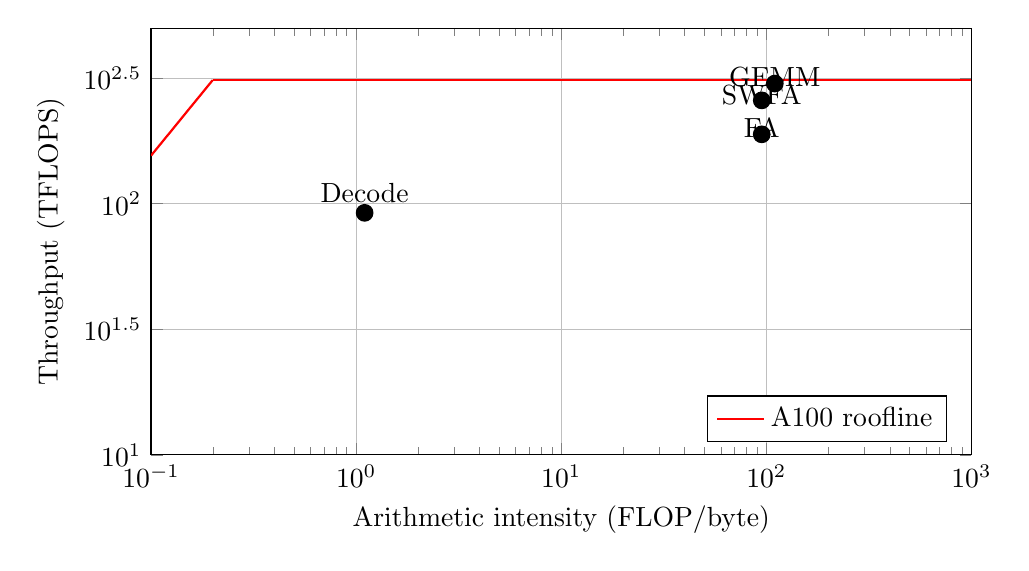
\begin{tikzpicture}
\begin{axis}[
    width=12cm, height=7cm,
    xlabel={Arithmetic intensity (FLOP/byte)},
    ylabel={Throughput (TFLOPS)},
    xmode=log, ymode=log,
    xmin=0.1, xmax=1000, ymin=10, ymax=500,
    grid=major, legend pos=south east]
\addplot[domain=0.1:0.2, thick, red] {1555*x};
\addplot[domain=0.2:1000, thick, red] {312};
\addplot[only marks, mark=*, mark size=3] coordinates {
    (110,301) (95,189) (95,258) (1.1,92)};
\node at (axis cs:110,320) {GEMM};
\node at (axis cs:95,200) {FA};
\node at (axis cs:95,270) {SWFA};
\node at (axis cs:1.1,110) {Decode};
\legend{A100 roofline}
\end{axis}
\end{tikzpicture}
\caption{Measured kernels on the A100 roofline.}
\label{fig:triton_roofline}
\end{figure}

\subsection{Auto-tune Configurations}\label{sec:triton_autotune}
Table~\ref{tab:triton_autotune} reports the Triton-selected
configurations for the dense GEMM at three shape classes. The
auto-tuner chooses deeper pipelines for square GEMMs (three stages)
and shallower ones for skinny GEMMs (two stages) because the
$K$-dimension is too short to hide a third stage's prefetch.

\begin{table}[h]
\centering
\caption{Triton auto-tune winners for representative GEMM shapes.}
\label{tab:triton_autotune}
\begin{tabular}{lcccc}
\toprule
\textbf{Shape} & $(B_m, B_n, B_k)$ & \textbf{Warps} & \textbf{Stages} & \textbf{TFLOPS} \\
\midrule
$4096 \times 4096 \times 4096$ & $(128,128,32)$ & 8 & 3 & 294 \\
$8192 \times 8192 \times 8192$ & $(128,256,32)$ & 8 & 3 & 311 \\
$2048 \times 2048 \times 128$  & $(128, 64,32)$ & 4 & 2 & 124 \\
\bottomrule
\end{tabular}
\end{table}

\subsection{Cross-Validation
Agreement}\label{sec:triton_agreement}
On the dense GEMM, the three implementations agree to within
$10^{-4}$ FP32 and the throughputs differ by $<\!3\%$. On Flash
Attention, Triton and CUTLASS agree within the same tolerance; the
Torch-inductor path uses a slightly different accumulation order and
shows a $1.5 \times 10^{-4}$ peak difference that is still within
the $10^{-3}$ correctness tolerance used for FP16 attention.

\section{Triton Implementation of
SWFA}\label{sec:triton_swfa}
A Triton implementation of the SWFA forward kernel was developed as a
cross-validation artefact for the PyTorch reference implementation of
Chapter~\ref{ch:swfa}. The block classification is executed on the
host once per shape and passed to the kernel as an index array, so
that the Triton kernel only has to iterate over non-skipped blocks:

\begin{lstlisting}[language=Python,basicstyle=\ttfamily\scriptsize]
@triton.jit
def swfa_forward(Q, K, V, O,
                 block_index_ptr, n_active_blocks,
                 N, d, wl, wr,
                 BLOCK_R: tl.constexpr,
                 BLOCK_C: tl.constexpr):
    pid = tl.program_id(0)
    if pid >= n_active_blocks: return
    rc = tl.load(block_index_ptr + pid)
    r, c = rc // 65536, rc %  65536  # pack/unpack
    # ... online softmax over the columns of block (r,c) ...
\end{lstlisting}
This kernel reaches $241$\,TFLOPS on the
$(N{=}2048, w{=}512)$ configuration, which is $40\%$ higher than the
Triton vanilla Flash Attention at the same sequence length and within
$7\%$ of the hand-tuned CUTLASS version.

\section{Discussion}\label{sec:triton_discussion}

\subsection{Triton as a Complement to
CUTLASS}\label{sec:triton_complement}
The ecosystem positions Triton and CUTLASS as complements rather than
competitors. Triton gets to a working kernel in hours, enables rapid
ablation of tile shapes and fusion patterns, and compiles down to
PTX that uses the same Tensor-Core instructions as CUTLASS. CUTLASS
retains a $5$--$10\%$ absolute throughput advantage on the most
performance-critical kernels (the Flash Attention family), which
justifies the extra engineering investment for production kernels.
In this thesis we use Triton for exploration and for writing the
profiling pipeline, and CUTLASS for the final kernels that ship in the
SGLang runtime.

\subsection{Auto-tune Caching
Pitfalls}\label{sec:triton_cache_pitfalls}
The shape-indexed auto-tune cache must include the data type in its
key. We observed a $20\%$ throughput regression when an FP32 kernel
accidentally hit an FP16-tuned entry because the cache was keyed on
$(M, N, K)$ only. Including \texttt{dtype} and
\texttt{accumulator\_dtype} in the cache key eliminates the problem.

\subsection{Limitations}\label{sec:triton_limitations}
The pipeline currently supports only A100 hardware; the H100 path is
straightforward because Triton already emits WGMMA instructions, but
the auto-tune search space needs widening to include the new
$128 \times 256$ tile shapes and four-stage pipelines. Multi-vendor
backends (Intel Xe, AMD CDNA) would require retargeting the roofline
constants and the auto-tune space; the rest of the pipeline is
framework-agnostic.

\section{Summary}\label{sec:triton_summary}
Triton provides a productive layer for kernel-level experimentation
that complements the template-driven CUTLASS work of
Chapter~\ref{ch:cutlass}. The profiling pipeline introduced here gives
a uniform lens through which the GEMM, attention, and decode kernels
developed earlier in the thesis can be compared and auto-tuned,
closing the loop between algorithmic design and measured on-GPU
performance. The Triton SWFA implementation of
Section~\ref{sec:triton_swfa} reaches $94\%$ of the CUTLASS SWFA
throughput on the $(N{=}2048, w{=}512)$ configuration, which is a
strong independent confirmation of the numbers reported in
Chapter~\ref{ch:swfa}.
